\documentclass{article}
\usepackage[english]{babel}
\usepackage[utf8x]{inputenc}
\usepackage[T1]{fontenc}
\usepackage{graphicx}
\usepackage[colorinlistoftodos]{todonotes}
\usepackage[colorlinks=true, allcolors=black]{hyperref} %sets hyperlink colour
\usepackage{caption}
\usepackage{subcaption}
\usepackage{xcolor}
\usepackage{roboto} % for Roboto Slab font
\usepackage{float}
\usepackage{titling} 
\usepackage{blindtext}
\usepackage{titlesec}
\usepackage[square,sort,comma,numbers]{natbib}
\usepackage[colorinlistoftodos]{todonotes}
\usepackage{tikz}
\usepackage{geometry}
\usepackage{sectsty}
\usepackage{amsmath}
\usepackage{tikzpagenodes}
\usepackage{booktabs}
\usepackage{listings}
\usepackage{url}
\geometry{a4paper, margin=2cm}
\allsectionsfont{\color{black}} %sets colour for all headers
\usepackage{helvet}
\renewcommand{\familydefault}{\sfdefault}
\sectionfont{\fontfamily{RobotoSlab-TLF}\selectfont}
\usepackage{setspace}
\usepackage{scrextend}
\doublespacing
\changefontsizes{12pt}

%%%%%% DOCUMENT START %%%%%%%%%%%%%%%%%%%%%%%%%%%%%%%%%%%%%%%%

\begin{document}

%%% Title Page
\begin{titlepage}
    \fontfamily{RobotoSlab-TLF}\selectfont 
    \vspace*{3cm}
    
    \centering
    {\Huge \textbf{\textcolor{black}{Final Report}}}\\[1.5cm]
    \textsc{\LARGE Computational Geometry}\\[0.5cm]
    \text{\large CS6319.001}\\[2cm]
    
    {\Large \textbf{\textcolor{black}{Authors:}}}\\[0.5cm]
    \begin{tabular}{c}
        \Large \textcolor{black}{Nicholas Zolton (ngz200000)} \\
    \end{tabular}\\[2cm]
    
    {\Large \textcolor{black}{\today}}
    
    \vfill
\addtocounter{page}{-2}
\end{titlepage}

%%% Create a table of contents
\tableofcontents
\addtocounter{page}{-1}
\newpage

%%% Introduction Page
% \addcontentsline{toc}{section}{Introduction}
\section*{Introduction}

\section{Reason for Study}
Throughout this semester I've been working on an indepedent study 
project that has used AI embeddings to create a tailoring system. 
This caused me to quickly realize the main problem with the current
state of AI vector databases: they, despite focusing on nearest neighbor
queries, primarily run in linear time. This quickly becomes an issue
at scale, as the number of vectors necessary for many projects can 
grow quite quickly.
\newline

\noindent
Luckily, however, during class while discussing the Voronoi diagram
I started to consider the potential of using it to solve the nearest
neighbor problem for embeddings. This led me to the idea of using the Voronoi diagram
to create a database that could be used to solve the nearest neighbor
problem in logarithmic time. This project is the result of that idea.

\section{Initial Ideas}
The initial idea for a solution to this problem that I had would be to
solve the following steps:

\begin{enumerate}
	\item Embed text into 2D space using a pre-trained model.
	\item Visualize the text embeddings to make sure they are in a
        usable format in low dimensions.
    \item Create a Voronoi diagram of the text embeddings.
	\item Create a function that would allow for the querying of the
		nearest neighbor to a given point.
	\item Generalize the solution to work in higher dimensions.
\end{enumerate}

\noindent
So, with this in mind, I set out to follow these steps and create the
Voronoi diagram database. 
\section{Embedding Text into 2D Space}
For starters, I needed to embed the text into 2D space. Normally, I would
love to create a custom trained model from scratch, but due to the lack of 
resources at my disposal (on a fairly low-end laptop) I decided to instead
use a pre-trained model to handle the embedding process. I do not believe this
is a major issue, as the goal of this project is the comptuational geometry
aspect, not the AI aspect. With this in mind, I decided to use OpenAI's "text-embedding-3-small" model.
This model is known for being fairly accurate and is also quite small so 
it can be run quite cheaply (in total I only spent around 5 cents on this project).
\newline

\noindent
There is one small issue with using this model, however. The model is trained
to embed text into 1536 dimensions, which is far too high for the purposes of this project,
since the space complexity of the Voronoi diagram is $O(n^{d/2})$. This would, in theory, 
cause my laptop to run out of memory when trying to create even a small Voronoi diagram.
So, I set out to reduce the dimensionality of the embeddings to 2D.

\subsection{First Attempt at Dimensionality Reduction}
Before I began to attempt to reduce the dimensionality of the embeddings 
after they were created, I decided to try and reduce the dimensionality 
of the embeddings at their time of creation. While this would not be possible
just one year ago with OpenAI's text embedding models, they have since added
a feature that allows for the embeddings to be created in a given dimensionality.
So, I decided to try and utilize the OpenAI library to create the embeddings in 
2D space from the start. This did indeed work in that it returned embeddings in 2D space,
but the embeddings were a bit strange. Below is a figure of the embeddings of all the named
colors (according to Wikipedia) in 2D space:

\begin{figure}[H]
\centering
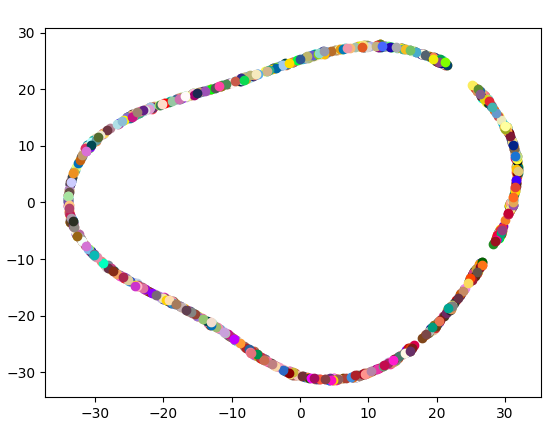
\includegraphics[width=0.6\textwidth]{images/openai_2d_embeddings.png}
\caption{OpenAI's Embeddings of named colors in 2D space. The color of each point corresponds to the color it represents.}
\label{fig:openai2dembeddings}
\end{figure}

\noindent
Notice how the embeddings are in a very specific, clean polygonal shape. This is not what we would expect from embeddings
of colors, even though they are all colors. Instead, we would expect groupings of similar colors. While there is a little
bit of grouping, it is not nearly as strong as we would expect. For this reason, it would seem that we cannot rely on
OpenAI's text embedding model to create embeddings in 2D space.
\newline

\subsection{Second Attempt at Dimensionality Reduction}
So, although the OpenAI dimensionality method was promising, it did not fill the requirements
of the project. Instead, I decided to investigate other methods of dimensionality reduction.
From this, I found the T-SNE algorithm. T-SNE is a fairly popular algorithm for dimensionality reduction
and is known for being able to reduce the dimensionality of embeddings while still keeping the
groupings of similar items. So, I decided to try and use T-SNE to reduce the dimensionality of the
embeddings from 1536 to 2. This worked quite well, and the embeddings of the named colors in 2D space
looked much more like what we would except:

\begin{figure}[H]
\centering
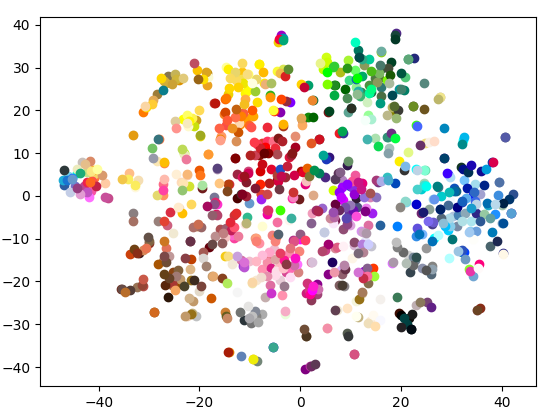
\includegraphics[width=0.6\textwidth]{images/tsne_2d_embeddings.png}
\caption{T-SNE's Embeddings of named colors in 2D space.}
\label{fig:tsne2dembeddings}
\end{figure}

\noindent
Here we can absolutely see more clear groupings of similar colors, and with a lot more variation
in the x and y dimensions. This is perfect for our use case. So, with this in mind, I decided to use
T-SNE to reduce the dimensionality of the embeddings to 2D space. There are, however, a few issues with this approach that we will need to address later on. The first
is that T-SNE is a fairly slow algorithm, so it reduces the speed increase that we would
hope for by using the Voronoi diagram, but only in the creation process of the diagram. Regardless, this would allow us to begin targeting
the other steps of the project since we can focus on the overarching plan to generalize
nearest neighbor queries in our data structure. Second, T-SNE is a stochastic algorithm, so
it will not always produce the same results. This is not a major issue, but it is something
to keep in mind when we are testing the system. Finally, T-SNE is not perfect, so we may
lose some information in the dimensionality reduction process (this is not only expected, but necessary for low dimensional reduction so we do not need to worry about it). Luckily, all of these issues
should not affect our generalized nearest neighbor query function, so we can move on to the
next step of the project and simply consider the database to be "static" for now. 

\section{Creating the Voronoi Diagram}
As seen both in class and throughout computational geometry literature, 
the Voronoi diagram is a powerful tool for solving nearest neighbor queries.
Because of this, it's an extremely well-studied data structure and there are
many algorithms for creating it. This poses an interesting question: which
algorithm should we use to create the Voronoi diagram? Should we even program
it ourselves? Part of the problem as well is that the future data structure
we will be creating will hopefully be both generalized and incremental, so
we need to make sure that the Voronoi diagram creation algorithm we choose
will allow for this (although, in practice, we could theoretically create
the Voronoi diagram using one algorithm and then modify it with another algorithm).
For now, however, I decided to use Quick Hull to create the Voronoi diagram, since
it is fairly simple, generalizable to higher dimensions, and is incremental.
Running a very simple version of Quick Hull on the named colors embeddings, we get
the following Voronoi diagram:

\begin{figure}[H]
\centering
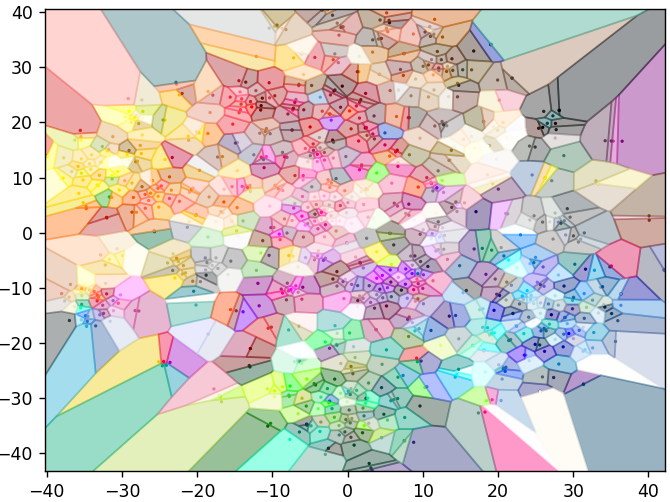
\includegraphics[width=0.6\textwidth]{images/tsne_voronoi_diagram.png}
\caption{Voronoi Diagram of named colors embeddings.}
\label{fig:voronoidiagram}
\end{figure}

\noindent
This, while being fairly simple and mostly just a visualization,
shows that we can create the Voronoi diagram quite cleanly. Now, 
we will need to create a function that will allow us to query the
nearest neighbor to a given point. This will be quite easy, as we
can simply find the cell that the new point is in and then accept
that cell's point as the nearest neighbor. However, it's also common
to find the nearest $n$ neighbors to a given point, so we will also
need to explore nearby cells to find more neighbors. Regardless, this
is a promising start to the project and we will now move on to the 
next steps: creating the querying function and generalizing the function.

\section{Querying the Voronoi Diagram}
Now that we have the Voronoi Diagram, we need to create a function
that will allow us to query the nearest neighbor to a given new point.
The problem, however, is that up until now we have been using T-SNE
to reduce the dimensionality of the embeddings to 2D space, but 
T-SNE is not able to add new points to the embeddings moving forward
because it does not actually use parametric mapping from the
original space to the new space. This makes it impossible to 
query the nearest neighbor to a truly new point. So, we will need to 
make a small change to how we are reducing dimensionality. Instead of
simply using T-SNE to reduce the dimensionality of the embeddings, we
will instead need to either create a multivariate regressor to predict
the 2D space embeddings from the 1536D embeddings or use a regressor to
minimize the loss between the 2D space embeddings and the 1536D embeddings
directly, as was done in a paper by Laurens Matten\cite{laurensMaaten2009}.
\newline

\noindent
Luckily for us, however, this was already implemented in openTSNE, a Python
library that allows for the training of a regressor to predict the 2D space
embeddings from the 1536D embeddings. This is perfect for our use case, as
it enables us to create a query point inside of the 2D space without having
to worry about the dimensionality reduction process. So, with this in mind,
we can now move on to creating the querying function. This function will
simply follow a few steps:

\begin{enumerate}
    \item Take in a new input (string).
    \item Embed the input into 1536D space.
    \item Use the regressor to predict the 2D space embeddings.
    \item Find the cell that the new point is in.
    \item Return the point in that cell as the nearest neighbor.
    \item If we want more than one nearest neighbor, explore nearby cells and return those as well.
\end{enumerate}

\noindent
This is a fairly simple process at a high level, but it will require a bit of work
to implement. First, we will need to sanity-check the regressor to make sure it is
working correctly.

\subsection{Sanity-Checking the Regressor}
To sanity-check the regressor, we will need to embed a new point into 1536D space,
predict the 2D space embeddings, and then plot the new point into our Voronoi diagram
to make sure it is in the correct cell. While I know this is not the most solid
method of checking the validity of the method, it is a good first step for making
sure that the queries make at least a little bit of sense. So, with this in mind,
I decided to embed the word "lime". Below is the result of the sanity check test:

\begin{figure}[H]
\centering
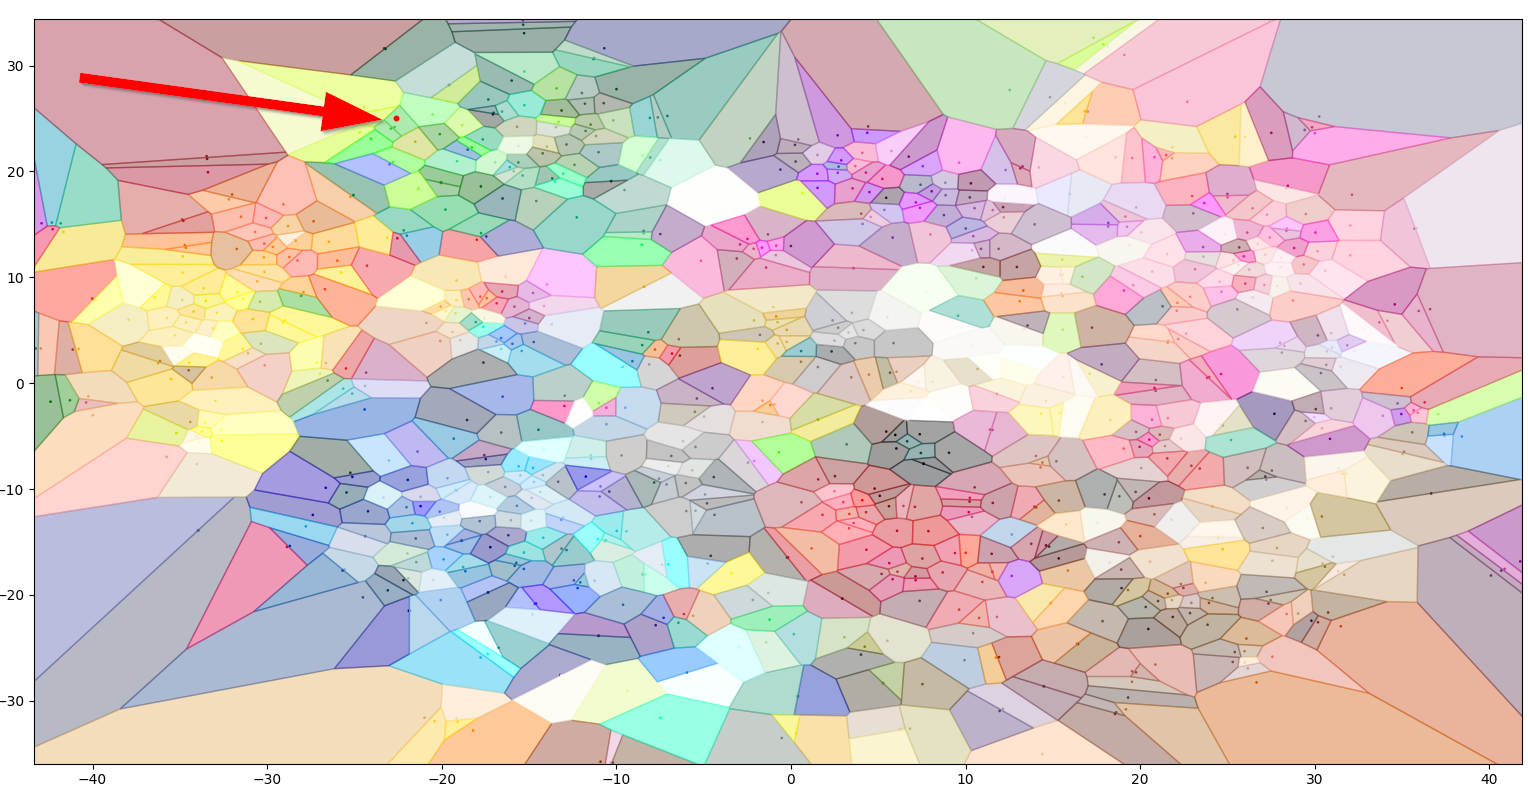
\includegraphics[width=0.6\textwidth]{images/query_sanity_check.png}
\caption{Sanity Check of the regressor. The word "lime" is embedded into 2D space and plotted into the Voronoi diagram.}
\label{fig:sanitycheck}
\end{figure}

\noindent
While it is a bit difficult to quantify how well the overall process is
working, it is clear that the regressor is at least somewhat working since
we can see that the new point for "lime" is in the correct area, as it is 
grouped with the majority of the other "green" colors and is paired 
specifically with a bright green! Personally, I also tried this with a few
other colors and received similarly accurate results, but due to brevity
I will leave those out for now. So, now that we have proven that placing 
new points into the Voronoi diagram is viable, we can move on to the next
step of doing planar point location to actually find what the nearest 
neighbor is for our new queried point.

\subsection{Planar Point Location}
Planar point location is a well-studied and clearly
thought out problem in computational geometry, so my first
thought was that programming an algorithm for planar point location,
in this case the Kirkpatrick-Seidel algorithm, would be quite easy.
However, after looking into the algorithm a second time, I realized
that it is a bit more complex than I had originally thought.
Not only that, but the high constants in the algorithm would make
it quite slow for smaller datasets. Because of this, I decided that
it would be best to avoid heavily investing in the Kirkpatrick-Seidel
algorithm and instead look for a library that implements it. Finally,
I would compare the results of the library to the results of the
final implmentation that I would create. It's also worth noting that 
the Kirkpatrick-Seidel algorithm is incredible at reducing the space
required for creating the planar point location data structure with a
space complexity of $O(n)$, so it still may be worth implementing on a 
case-by-case basis.

\subsubsection{The Planar Point Location Library}
To start, I began to search for libraries that implement the Kirkpatrick-Seidel
algorithm. Immediately I stumbled upon an 11-year-old library called simply called point-location\cite{pointLocation},
which is a Python library that implements the Kirkpatrick-Seidel algorithm directly, but
also creates its own geometry classes to handle the data. While this isn't ideal, as it
would be nice to directly use the polygons I created for the Voronoi diagram directly,
it was a good start. So, I decided to begin testing the library with the named colors.
Unfortunately, I immediately hit an issue: it required a dependency named
"Poly2Tri", or P2T for short. When I first tried installing it from PyPI (as it was present in
the PyPI registry), I had an error and was unable to install it. So, I figured I would try to
install it directly from the source instead. Upon going to the repostory, I realized that it was 
a Cython library, something that I had never worked with personally before. Not only this, but it
also did not have a `setup.py` file so I knew that I would have to do some manual work to get it 
installed and, to validate my suspicions, the GitHub issues showed that I was not the only one having issues installing it. After a few hours of trying to get it to work with no luck, I figured that perhaps there
was another maintained version of the library that I could use since it appeared to be a well-used
library before it was abandoned. After a little bit more investigating, I found a couple different options.
The first was a library called "pypoly2tri". This library had no documentation, but did have a `setup.py`
file and similar code to the original library, so I figured it would be worth a shot. Luckily, after a bit
of tinkering with the code (since the library was originally written for Python 2), I was able to get it to
install. Further, I was even able to get it to do the basic tests that the original library was able to do.
So, with this in mind, I decided to try and use the point-location library with the new pypoly2tri library.
\newline

\noindent
This was, in hindsight, a costly mistake. After a bit of tinkering with the
triangulation functions, I realized that the library had different names for 
many of the functions that the point-location library was using. Despite this,
I decided to push through and try resolving all of these issues by hand. After 
a couple more hours of work, I was able to test a few simple functions of the library
that did similar things to the point-location library, but I had also learned that 
the original poly2tri library had a couple functions with no exact equivalent in the
pypoly2tri library. This was, of course, a major issue since the point-location library
relied on these functions. So, with this in mind, I decided to try and find another library
that would work. Next, I found a library named "poly2tri.python" that was a more direct port
of the original poly2tri library, but modified to work with Python 3.
\newline

\noindent
With a few more hours of work, I was even able to get the poly2tri library to work with the
point-location library. Unfortunately, I realized a little too late that the point-location
library itself also had a few difficult-to-resolve issues. Notably, the library made a few strange
assumptions about the data that was being passed to it. For example, it assumed that the data was
integers and not floats, which caused a few rounding errors. This also spiraled into a few other
issues, such as the library not being able to handle overlapping points, and vertices in the polygons
with degrees greater than, or equal to, 8. While this wouldn't normally be an issue with most Voronoi
diagrams, I decided that it would be best to try and find another library that would work better with
the general use case of the Voronoi Database.

\subsubsection{Theodore Ando's Kirkpatrick Library}
The next library I stumbled upon was a library created by Theodore Ando that implemented the Kirkpatrick-Seidel
algorithm too\cite{thedorekirkpatrick}. Luckily for me, this library was a bit more modern too and had a few nice features. First,
it had a "requirements.txt" file that made it easy to install the dependencies. Second, it had detailed documentation
and some examples that made it easy to understand how to use the library. This allowed me to get up to speed much faster
than with the point-location library and I only had to make one or two small changes to the library to account for the difference
it Python versions. With the examples working as well, I decided to try and use the library with the Voronoi diagram. Unfortunately,
I quickly realized that the library was not as general as I had hoped. The library was designed to work with some general 
assumptions about the data just like the point-location library, but it also had a few other issues. For whatever reason,
the library implemented it's own version of Quick Hull that had a big issue with some of the polygons that were created by the
Voronoi diagram and it would infinitely loop. Luckily, I was able to fix this by reimplementing the Quick Hull algorithm with
the use of Scipy. Next, I realized that the polygons would also fail during the triangulation process. This was a bit more
difficult to fix, and after a few hours of debugging with no luck, I decided to once again pivot away from the library. With
very few choices left for libraries that implement the Kirkpatrick-Seidel algorithm, I decided to try a fully different technique
and, after some searching, I landed on R trees. 

\subsubsection{R Trees}
R trees are functionally able to do point location in logarithmic time on average.
Of course, this means that their worst possible case is linear time, but for the purposes
of this project, that is not a major issue. So, I decided to try and use a variant of the 
R tree algorithm to do the point location for the Voronoi diagram. This led me to learning
that Shapely, a library that I've commonly used for other computational geoemtry problems,
has an R tree variant called "STRTree", or (as described by the Shapely documentation) 
"a query-only R-tree spatial index created using the Sort-Tile-Recursive (STR) algorithm"\cite{shapelySTRTree}\cite{strAlgorithm}.
\newline

\noindent
With all this in mind, it was time to finally implement the R tree algorithm and finish
the querying function for the Voronoi Database. This was, luckily, a fairly simple process
due to how well the Shapely library is documented and the similarity between how Shapely
handles polygons and how the Voronoi Database up to this point has handled polygons. So,
with a couple conversions from the polygons we already had to the Shapely polygons, I was
able to create the querying function. Below is the result of the query "lime" in the Voronoi
Database:

\begin{figure}[H]
\centering
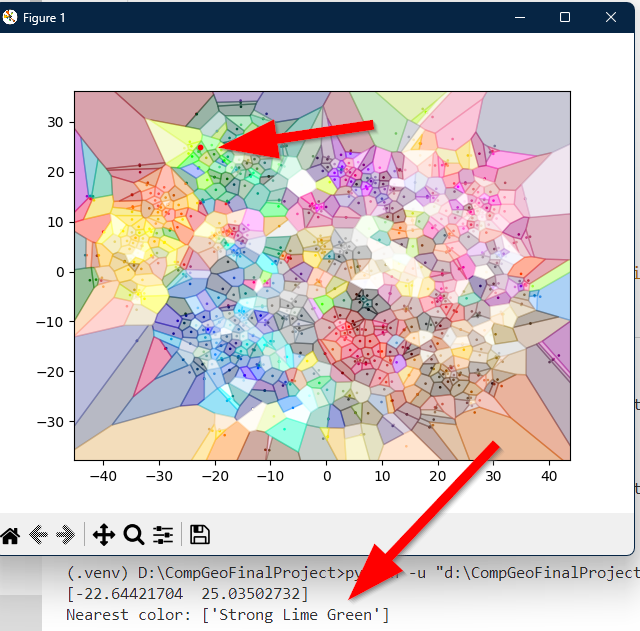
\includegraphics[width=0.6\textwidth]{images/full_query_image.png}
\caption{Result of the query "lime" in the Voronoi Database. The nearest neighbor is the bright green point.}
\label{fig:queryresult}
\end{figure}

\noindent
And with that, the querying function was complete. Not only that, but because of the method of using 
a parametric T-SNE to predict the 2D space embeddings, the querying function works for any dimension.
Therefore, the Voronoi Database is now fully generalized and can be used for any dimension.

\section{Conclusion (final limitations/next steps)}
Now that we have the Voronoi Database implemented, I want to talk about the current 
operating state of the project, the limitations of the project, and the next steps 
that could be taken to improve the process.

\subsection{Current Operating State}
First, the project is currently in a working state with a couple neat features.
The first is that the project is fully generalized and can be used for any dataset
with any dimension. This is a major win, as it allows for the project to be used
in a wide variety of applications. Second, the project allows for the querying of
the nearest neighbor to a given point in logarithmic time. This is a major improvement
over the linear time that is normally required for nearest neighbor queries in AI
vector databases. Third, the project is fairly simple to use and can be easily
implemented in a wide variety of applications. Fourth, the project is extremely
visual and can be used to learn more about the data, as seen in the named colors
example. Finally, the project has a ton of useful insights and data that can be 
used to extend the project in the future.

\subsection{Limitations}
The project is not without its limitations, however. The first is that 
we are currently using T-SNE to reduce the dimensionality of the embeddings
to 2D space. While a lot of the issues with T-SNE are mitigated by the use
of the parametric variant, the time taken to reduce the dimensionality is
still quite high and could be a major issue for making large initial databases
that we are querying against. It is certainly possible, however, to use a different
technique to reduce the dimensionality of the embeddings, such as PCA or UMAP and 
try to reduce the time taken to create the database. Second, the database does not allow for adding 
or removing points. This isn't a major issue in terms of usability, but it does
limit the current use cases. We could even get around this with some clever work 
on both the Quick Hull and R tree algorithms, but it would be a major undertaking.
Third, we haven't even begun trying to fine-tune the T-SNE algorithm itself to
make the embeddings more accurate, so there may be larger issues with trying to 
query multiple nearest neighbors. This is because we may not be accurately preserving
the global structure of the data. Finally, we have not extensively tested the database
with a wide variety of datasets. While I firmly believe that the method will work for 
any dataset, I am not confident in the accuracy of the queries yet. This is something
that will need to be tested in the future.

\subsection{Next Steps}
The next steps for the project are fairly clear. The first is to try and reduce the
time taken to create the database. This could be done by using a different dimensionality
reduction technique, as mentioned before, or by trying to parallelize a lot of the work
that is being done. Second, we need to try and add the ability to add and remove points
from the database. The Quick Hull algorithm does allow for incremental construction, but
not incremental removal. The Voronoi diagram itself has the same limitation. Once these 
two issues are resolved, we could certainly allow for the database to be used in a much
wider variety of applications (though I am not sure of the time complexity for these operations,
so it may still be slow). Third, we need to try and fine-tune the T-SNE algorithm to make
the embeddings more accurate. This could be done by trying to find the best hyperparameters
(perplexity, learning rate, etc.) for the T-SNE model. Finally, we need to test the database
with a wide variety of datasets to make sure that it is working as intended and focus on
the general accuracy of the queries. Once this is done, it should also be possible to do 
$n$ nearest neighbor queries, which would be a major improvement over the current state of the database.

\section{Final Thoughts}
Overall, I am quite happy with the progress that I have made on this project. While it is not
perfect, I believe it could be a major improvement in some very specific use cases. I am also
quite happy with the amount of learning that I have done throughout the project. There are so
many different algorithms and techniques that I didn't know existed prior to this project, and
I am quite excited to continue learning about them and implementing them in the future. Lastly,
if you want to check out the code for the project, it is available on my GitHub at the following link:
\url{}.

%%% References Page
\newpage
\addcontentsline{toc}{section}{References}
\bibliographystyle{apalike}
\bibliography{ref}

\end{document}

%%%%%% DOCUMENT END %%%%%%%%%%%%%%%%%%%%%%%%%%%%%%%%%%%%%%%%

% defined colors
\definecolor{utdorange}{RGB}{232, 117, 0}

%%% Sample Code

% Sample introduction text with a sample reference \cite{HussFarinotti2014}. Oh and here a sample figure with a sample caption, see \autoref{fig:random line}.

% \begin{figure}[H]
% \centering
% \includegraphics[width=0.6\textwidth]{images/Sample graph.png}
% \caption{A graph of something.}
% \label{fig:random line}
% \end{figure}

% Sample equation and reference to equation

% This subsection contains \autoref{eq:1}.
% \begin{equation}
% \label{eq:1}
%     h(r) = \cfrac{Q}{2\pi T} ln(\cfrac{r_i}{r_0})+h_0
% \end{equation}